% This file was created by matlab2tikz.
%
%The latest updates can be retrieved from
%  http://www.mathworks.com/matlabcentral/fileexchange/22022-matlab2tikz-matlab2tikz
%where you can also make suggestions and rate matlab2tikz.
%
\documentclass[]{standalone}
\usepackage{amsmath}
\usepackage{graphicx}
\usepackage[pdf]{pstricks}
\usepackage{pgfplots}
\pgfplotsset{compat=newest}
\usepgfplotslibrary{fillbetween}
%% the following commands are needed for some matlab2tikz features
\usetikzlibrary{plotmarks}
\usetikzlibrary{arrows.meta}
\usepgfplotslibrary{patchplots}
\usetikzlibrary{decorations.text}
\usetikzlibrary{shapes.multipart}


\newcommand{\logLogSlopeTriangle}[5]
{
	% #1. Relative offset in x direction.
	% #2. Width in x direction, so xA-xB.
	% #3. Relative offset in y direction.
	% #4. Slope d(y)/d(log10(x)).
	% #5. Plot options.
	
	\pgfplotsextra
	{
		\pgfkeysgetvalue{/pgfplots/xmin}{\xmin}
		\pgfkeysgetvalue{/pgfplots/xmax}{\xmax}
		\pgfkeysgetvalue{/pgfplots/ymin}{\ymin}
		\pgfkeysgetvalue{/pgfplots/ymax}{\ymax}
		
		% Calculate auxilliary quantities, in relative sense.
		\pgfmathsetmacro{\xArel}{#1}
		\pgfmathsetmacro{\yArel}{#3}
		\pgfmathsetmacro{\xBrel}{#1-#2}
		\pgfmathsetmacro{\yBrel}{\yArel}
		\pgfmathsetmacro{\xCrel}{\xArel}
		%\pgfmathsetmacro{\yCrel}{ln(\yC/exp(\ymin))/ln(exp(\ymax)/exp(\ymin))} % REPLACE THIS EXPRESSION WITH AN EXPRESSION INDEPENDENT OF \yC TO PREVENT THE 'DIMENSION TOO LARGE' ERROR.
		
		\pgfmathsetmacro{\lnxB}{\xmin*(1-(#1-#2))+\xmax*(#1-#2)} % in [xmin,xmax].
		\pgfmathsetmacro{\lnxA}{\xmin*(1-#1)+\xmax*#1} % in [xmin,xmax].
		\pgfmathsetmacro{\lnyA}{\ymin*(1-#3)+\ymax*#3} % in [ymin,ymax].
		\pgfmathsetmacro{\lnyC}{\lnyA+#4*(\lnxA-\lnxB)}
		\pgfmathsetmacro{\yCrel}{\lnyC-\ymin)/(\ymax-\ymin)} % THE IMPROVED EXPRESSION WITHOUT 'DIMENSION TOO LARGE' ERROR.
		
		% Define coordinates for \draw. MIND THE 'rel axis cs' as opposed to the 'axis cs'.
		\coordinate (A) at (rel axis cs:\xArel,\yArel);
		\coordinate (B) at (rel axis cs:\xBrel,\yBrel);
		\coordinate (C) at (rel axis cs:\xCrel,\yCrel);
		
		% Draw slope triangle.
		\draw[#5]   (A)-- node[pos=0.5,anchor=north] {1}
		(B)-- 
		(C)-- node[pos=0.5,anchor=west] {#4}
		cycle;
	}
}
\begin{document}
	
	
	
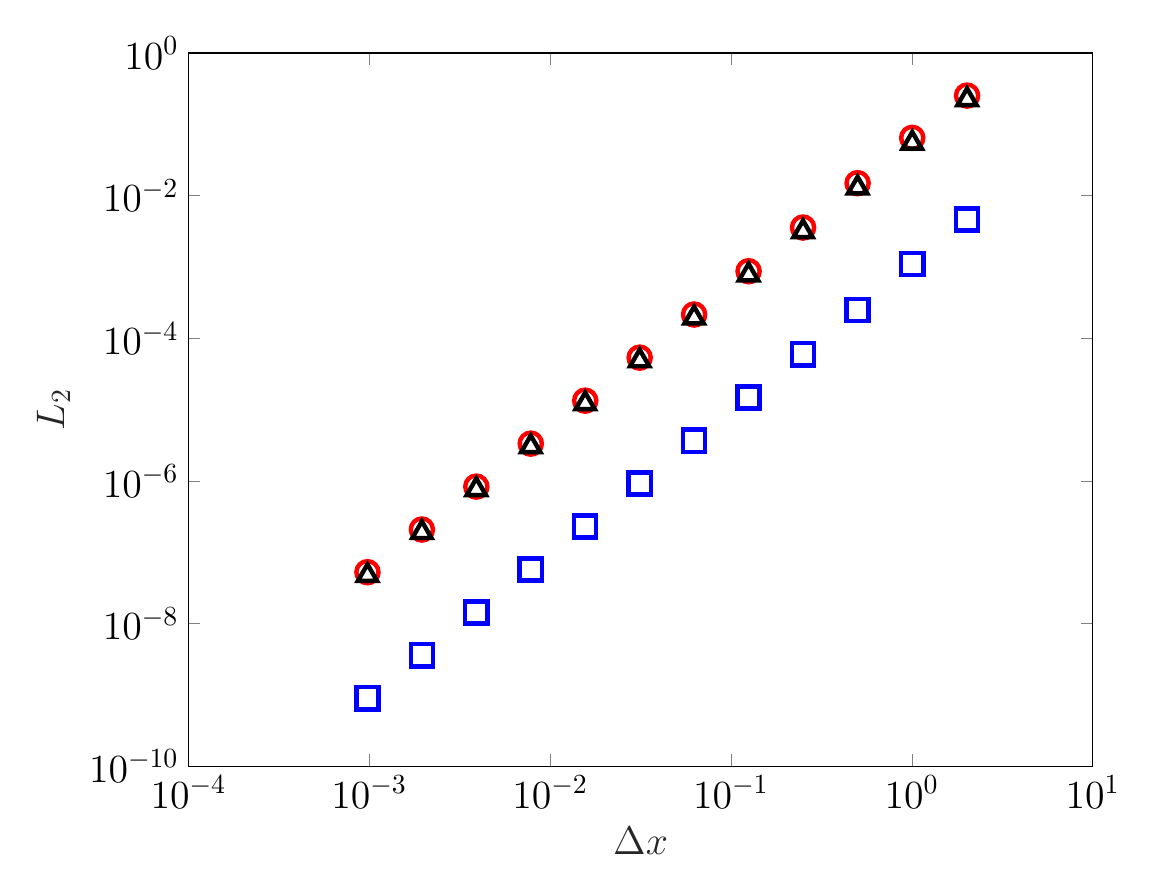
\begin{tikzpicture}
\tikzstyle{every node}=[font=\Large]
\begin{axis}[%
width=4.521in,
height=3.566in,
at={(0.758in,0.481in)},
every axis plot/.append style={ultra thick},
scale only axis,
xmode=log,
xmin=0.0001,
xmax=10,
xtick={0.0001,  0.001,   0.01,    0.1,      1,     10},
xminorticks=false,
xlabel style={font=\color{white!15!black}},
xlabel={\Large $\Delta x$},
ymode=log,
ymin=1e-10,
ymax=1,
ytick={ 1e-10,  1e-08,  1e-06, 0.0001,   0.01,      1,    100},
yminorticks=false,
ylabel style={font=\color{white!15!black}},
ylabel={\Large $L_2$},
axis background/.style={fill=white},
legend style={at={(0.03,0.97)}, anchor=north west, legend cell align=left, align=left, draw=white!15!black}
]
 \logLogSlopeTriangle{0.6}{0.2}{0.16}{2}{black};

\addplot [color=blue, draw=none, mark=square, mark size=4pt, mark options={solid, blue}]
  table[row sep=crcr]{%
2.02020202020202	0.00463841144255584\\
1.00502512562814	0.00109462848612723\\
0.50125313283208	0.000249513007616719\\
0.250312891113892	5.97277770421127e-05\\
0.125078173858662	1.47403356072022e-05\\
0.0625195373554236	3.67476742576749e-06\\
0.0312548835755587	9.18421547530889e-07\\
0.0156262207984999	2.29629553717499e-07\\
0.00781280518770264	5.74151904488804e-08\\
0.00390632629543546	1.43549234597775e-08\\
0.00195314407367259	3.58974140559057e-09\\
0.000976567268394865	8.96825760025487e-10\\
};
%\addlegendentry{h}

\addplot [color=red, draw=none, mark=o, mark size=4pt, mark options={solid, red}]
  table[row sep=crcr]{%
2.02020202020202	0.253157663984495\\
1.00502512562814	0.0646556964993866\\
0.50125313283208	0.0149700304714129\\
0.250312891113892	0.00357472150000761\\
0.125078173858662	0.000872407439409657\\
0.0625195373554236	0.000215560122624255\\
0.0312548835755587	5.36036745398622e-05\\
0.0156262207984999	1.33678801566722e-05\\
0.00781280518770264	3.33806249395967e-06\\
0.00390632629543546	8.3403050896899e-07\\
0.00195314407367259	2.08518642545866e-07\\
0.000976567268394865	5.2595539208592e-08\\
};
%\addlegendentry{G}

\addplot [color=black, draw=none, mark=triangle, mark size=4pt, mark options={solid, black}]
  table[row sep=crcr]{%
2.02020202020202	0.222869253649656\\
1.00502512562814	0.054720939845086\\
0.50125313283208	0.012899450324837\\
0.250312891113892	0.0031361593007678\\
0.125078173858662	0.00077793390370012\\
0.0625195373554236	0.000194217029144629\\
0.0312548835755587	4.85590428439022e-05\\
0.0156262207984999	1.21423971226173e-05\\
0.00781280518770264	3.03611181250639e-06\\
0.00390632629543546	7.59089124947063e-07\\
0.00195314407367259	1.89822792345145e-07\\
0.000976567268394865	4.74645021868212e-08\\
};
%\addlegendentry{u}

\end{axis}
\end{tikzpicture}%
\end{document}